\subsection{Model analityczny}

\begin{adjustwidth}{2em}{0pt}
Zostanie przedstawiona analiza systemu wraz z diagramem klas, diagramem typu robustness oraz diagramem sekwencji.
\end{adjustwidth}

\subsubsection{Model pojęciowy - diagram klas}


\begin{adjustwidth}{5em}{0pt}

\begin{figure}[H]
    \centering
    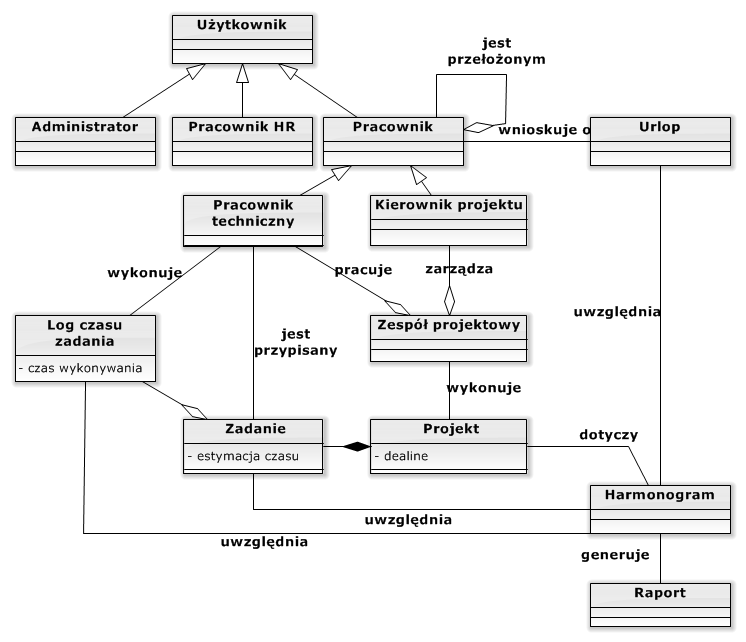
\includegraphics[scale=0.9]{diagramy/modelKlas/Classdiagram2.png}
    \caption{Analityczny diagram klas - zbiór pojęć}
    \label{fig:zbior_pojec}
\end{figure}

Powyższy diagram przedstawia zestaw pojęć opisujących analityczną część projektu. Pokzana jest struktura relacji i role pracowników, gdzie istnieje kilka typów aktorów. Wspomniania funkcja przestawiania relacji hierarchii w firmie dotyczy jedynie pracowników, którzy są kierownikami projektu, bądź pracownikami technicznymi. W ramach danego projektu powstaje zespół projektowy, jednak każdy z pracowników może uczestniczyć w wielu projektach. Na harmonogram wpływają zarówno estymacje zadań w projekcie, czas dotychczasowy przepracowany w ramach zadania, oraz urlopy. Daje to możliwość elastycznego planowania, oraz raportowania w sytuacjach kryzysowych dla projektu.

\end{adjustwidth}

\subsubsection{Stereotypowy diagram klas}
\begin{adjustwidth}{5em}{0pt}

\begin{figure}[H]
    \centering
    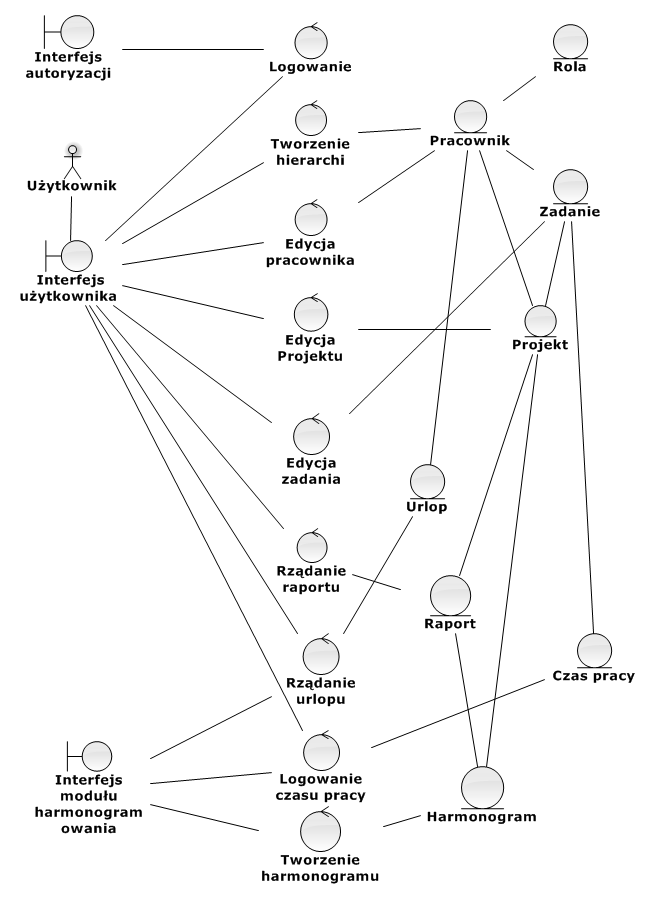
\includegraphics[scale=0.8]{diagramy/modelKlas/Robustnessdiagram1.png}
    \caption{Stereotypowy diagram klas - logika działania systemu}
    \label{fig:logika}
\end{figure}

\begin{figure}[H]
    \centering
    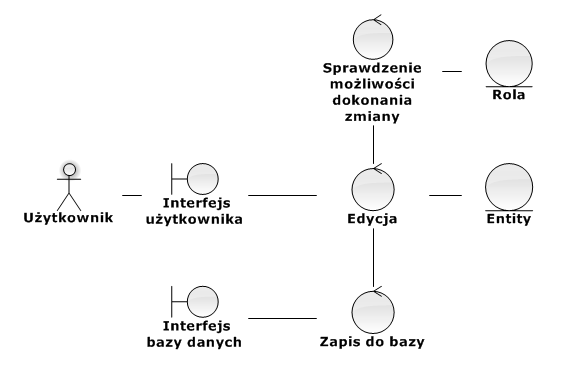
\includegraphics[scale=0.8]{diagramy/modelKlas/Robustnessdiagram2.png}
    \caption{Stereotypowy diagram klas - model ogólny uwzględniający sprawdzanie ról użytkownika}
    \label{fig:ogolny}
\end{figure}

\end{adjustwidth}
